% Created 2019-02-07 jeu. 19:41
% Intended LaTeX compiler: pdflatex
\documentclass[11pt]{article}
\usepackage[utf8]{inputenc}
\usepackage[T1]{fontenc}
\usepackage{graphicx}
\usepackage{grffile}
\usepackage{longtable}
\usepackage{wrapfig}
\usepackage{rotating}
\usepackage[normalem]{ulem}
\usepackage{amsmath}
\usepackage{textcomp}
\usepackage{amssymb}
\usepackage{capt-of}
\usepackage{hyperref}
\usepackage{minted}
\usepackage[french]{babel}
\usepackage[x11names]{xcolor}
\hypersetup{linktoc = all, colorlinks = true, urlcolor = DodgerBlue4, citecolor = PaleGreen1, linkcolor = black}
\author{Raoul HATTERER}
\date{\today}
\title{Traitement d'image avec commentaires\\\medskip
\large (compléments d'informations à destination du professeur)}
\hypersetup{
 pdfauthor={Raoul HATTERER},
 pdftitle={Traitement d'image avec commentaires},
 pdfkeywords={},
 pdfsubject={},
 pdfcreator={Emacs 26.1 (Org mode 9.2)}, 
 pdflang={French}}
\begin{document}

\maketitle
\tableofcontents

Source : \href{http://www.ac-grenoble.fr/disciplines/informatiquelycee/n\_site/snt\_photo\_transImg.html}{Traitement d'image de l'académie de grenoble}

\section{Installation de PIL}
\label{sec:orge25863d}

À faire au préalable par le professeur.

\begin{minted}[]{shell}
 pip3 install pillow
\end{minted}



\section{Codage RVB et niveau de gris}
\label{sec:orgfba8e4a}

Aller sur \href{https://www.w3schools.com/colors/colors\_rgb.asp}{colors RGB} et tester ce que l'on obtient si l'on remplace chacune des valeurs R, V et B d'un pixel par la moyenne des sous-pixels.
Essayer pour plusieurs couleurs.

\section{Image de départ}
\label{sec:org3c6010e}

\begin{figure}[htbp]
\centering
\includegraphics[width=.9\linewidth]{pomme.jpg}
\caption{Image de départ (480px \texttimes{} 300px)}
\end{figure}


\section{Comment lire un pixel}
\label{sec:orgf8ac23b}

Après avoir fait quelques recherches sur ce qu'est un "pixel", voyons comment lire le pixel de coordonnées (100,250).

\begin{minted}[]{python}
from PIL import Image
img = Image.open("pomme.jpg")
r,v,b=img.getpixel((100,250))
print("canal rouge : ",r,"canal vert : ",v,"canal bleu : ",b)
\end{minted}

\begin{verbatim}
canal rouge :  19 canal vert :  88 canal bleu :  192
\end{verbatim}


\section{Comment écrire un pixel}
\label{sec:org019f0a7}

\begin{minted}[]{python}
from PIL import Image
img = Image.open("pomme.jpg")
img.putpixel((5,5),(255,0,0))
img.show()
\end{minted}


\section{Que fait le programme suivant ?}
\label{sec:orgb906dce}

\begin{minted}[]{python}
from PIL import Image                        # Importation de la librairie PILLOW (gestion image)
img = Image.open("pomme.jpg")                # Mise en mémoire dans la variable "img" du fichier pomme.jpg qui doit être dans le même répertoire que le programme
largeur_image,hauteur_image=img.size         # Méthode size aplliquée à la variable img qui renvoie la largeur et la hauteur de l'image

for y in range(hauteur_image):               # Boucle pour parcourir les toutes les lignes
    for x in range(largeur_image):           # Boucle inbriquée pour parcourir les pixels de la ligne en cours
        rouge,vert,bleu=img.getpixel((x,y))  # Méthode getpixels appliquée à la variable img qui renvoie les valeurs r,g,b du pixel à la position x,y
        nouveau_rouge=vert                   # Le vert devient rouge
        nouveau_vert=bleu                    # Le bleu devient vert
        nouveau_bleu=rouge                   # Le rouge devient bleu
        img.putpixel((x,y),(nouveau_rouge,nouveau_vert,nouveau_bleu)) # Méthode putpixel qui remplace les valeurs R, V, B du pixel à la position x,y 

img.show()                                   # Affichage de l'image
img.save("pommeMystere.jpg")                 # Sauvegarde de l'image obtenue
\end{minted}


On analyse le code ci-dessus qui servira de base pour le défi suivant.

\begin{figure}[htbp]
\centering

\includegraphics[width=.9\linewidth]{pommeMystere.jpg}
\caption{Résultat du programme mystère}
\end{figure}


\section{Passage d'une image en niveau de gris}
\label{sec:org7bb459f}

Après avoir fait quelques recherches sur les "images en niveau de gris", écrivez un programme qui transforme une "image couleur" en une "image en niveau de gris".

Petite astuce qui pourrait vous aider : en Python pour avoir une division entière (le résultat est un entier), il faut utiliser l'opérateur // à la place de l'opérateur / 

Remarque: On donne l'algorithme aux élèves (ou on le construit avec eux) ; ils doivent alors programmer le passage d'une image couleur à une image en niveaux de gris.


\begin{minted}[]{python}
from PIL import Image
img = Image.open("pomme.jpg")
largeur_image=480
hauteur_image=300

for y in range(hauteur_image):
    for x in range(largeur_image):
       rouge,vert,bleu=img.getpixel((x,y))
       nouveau_rouge=(vert+bleu+rouge)//3
       nouveau_vert=(vert+bleu+rouge)//3
       nouveau_bleu=(vert+bleu+rouge)//3
       img.putpixel((x,y),(nouveau_rouge,nouveau_vert,nouveau_bleu))

img.show()
img.save("pommegrise.jpg")
\end{minted}

\begin{figure}[htbp]
\centering
\includegraphics[width=.9\linewidth]{pommegrise.jpg}
\caption{Image en niveaux de gris}
\end{figure}


\section{Passage d'une image en vrai niveau de gris (sans informations triplées)}
\label{sec:org1941b7e}


\subsection{Utilisation du mode \texttt{L} (luminance) pour les images en nuances de gris=}
\label{sec:org6b27ac4}

\begin{minted}[]{python}
from PIL import Image
img = Image.open("pomme.jpg").convert("L")
img.show()
img.save("pommegriseL.jpg")
\end{minted}

Comparer la taille des différents fichiers. Conclure.

\begin{figure}[htbp]
\centering

\includegraphics[width=.9\linewidth]{pommegriseL.jpg}
\caption{Image en niveaux de gris (sans redondance)}
\end{figure}


\emph{Réponse : code sur un octet par pixel l'image prend moins de place donc le fichier est moins lourd. Remarque : Pas trois fois moins lourd ; notamment car le format jpeg est compressé.}

\subsection{Existe-t-il d'autres modes ?}
\label{sec:org22a6150}

Les \href{https://pillow.readthedocs.io/en/latest/handbook/concepts.html\#modes}{modes} supportés par \texttt{Pillow} sont : 

\begin{itemize}
\item \texttt{1} (1-bit pixels, black and white, stored with one pixel per byte)
\item \texttt{L} (8-bit pixels, black and white)
\item \texttt{P} (8-bit pixels, mapped to any other mode using a color palette)
\item \texttt{RGB} (3x8-bit pixels, true color)
\item \texttt{RGBA} (4x8-bit pixels, true color with transparency mask)
\item \texttt{CMYK} (4x8-bit pixels, color separation)
\item \texttt{YCbCr} (3x8-bit pixels, color video format)
\item \texttt{LAB} (3x8-bit pixels, the L*a*b color space)
\item \texttt{HSV} (3x8-bit pixels, Hue, Saturation, Value color space)
\item \texttt{I} (32-bit signed integer pixels)
\item \texttt{F} (32-bit floating point pixels)
\end{itemize}



\section{Pour aller plus loin}
\label{sec:org0d16e07}

\subsection{Créer une image en négatif}
\label{sec:org4daf353}

\begin{minted}[]{python}
from PIL import Image
img = Image.open("pomme.jpg")
largeur_image,hauteur_image=img.size

for y in range(hauteur_image):
    for x in range(largeur_image):
        rouge,vert,bleu=img.getpixel((x,y))
        nouveau_rouge=255-rouge
        nouveau_vert=255-vert
        nouveau_bleu=255-bleu
        img.putpixel((x,y),(nouveau_rouge,nouveau_vert,nouveau_bleu))

img.show()
img.save("pommeNegatif.jpg")
\end{minted}

\begin{figure}[htbp]
\centering
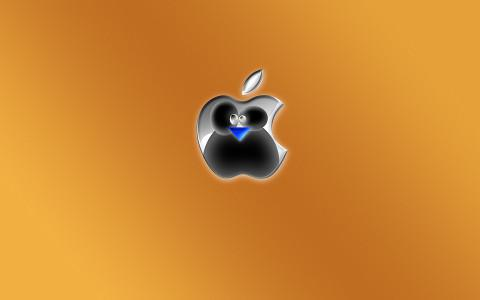
\includegraphics[width=.9\linewidth]{pommeNegatif.jpg}
\caption{Négatif}
\end{figure}

\subsection{Diagonale}
\label{sec:org51b03b7}

Créer le programme qui garde l'image d'origine au-dessus d'une diagonale et qui transforme en niveau de gris en-dessous

\begin{minted}[]{python}
from PIL import Image
img = Image.open("pomme.jpg")
largeur_image,hauteur_image=img.size

for y in range(hauteur_image):
    tailleDiag=int((largeur_image/hauteur_image)*y)
    for x in range(tailleDiag):
        r,v,b=img.getpixel((x,y))
        n_r=(v+b+r)//3
        n_v=(v+b+r)//3
        n_b=(v+b+r)//3
        img.putpixel((x,y),(n_r,n_v,n_b))

img.show()
img.save("pommemisgrise.jpg")
\end{minted}

\begin{center}

\includegraphics[width=.9\linewidth]{pommemisgrise.jpg}
\end{center}
\end{document}